\documentclass[11pt]{article}
\usepackage{xcolor}
\usepackage{graphicx}
\usepackage{float}

\title{Microcontroller Basics} % in C/C++}
\author{UQMARS}
\date{\today}

\begin{document}
\maketitle
\pagebreak
\section*{Microcontroller Developement Board options}
\begin{itemize}
    \item Arduino Family
    \begin{itemize}
        \item Arduino Uno (ATmega328P)
        \item Arduino Mega (ATmega2560)
        \item Ardiono Nano (ATmega328P)
    \end{itemize}
    \item Raspberry Pi Family 
    \begin{itemize}
        \item Raspberry Pi Model B
        \item Raspberry Pi Zero
        \item Raspberry Pi Pico
    \end{itemize}
    \item Espressif Family
    \begin{itemize}
        \item ESP8266 Development Boards
        \item ESP32 Development Boards
    \end{itemize}
\end{itemize}

\subsection*{How to choose your board} 
The best way to choose the board that suits you is to fully analyse what you need the board for. Knowing your use case will allow you put constraints on various factors such as cost, size, number of GPIO pins, power usage, memory ..

\section*{Basic Microcontroller Programming - Intro to the Arduino IDE}

\subsection*{Introduction to IDE}
Installing Arduino IDE from website.\\
Checking whether you can find your board - Install CP2102 USB to UART Bridge Driver\\
Adding the ESP32 Add-on to the Arduino IDE\\
Introduce the IDE what the power it offers. Such as Serial Monitor ...\\
Introduce basics of setup and block loop {}\\

\subsection*{Simple Blink LED}
Blinking an LED is the equivalent to hello world in the embedded world. The figure below shows how the LED can be wired to a GPIO pin. 
\begin{figure}[H]
  \centering
  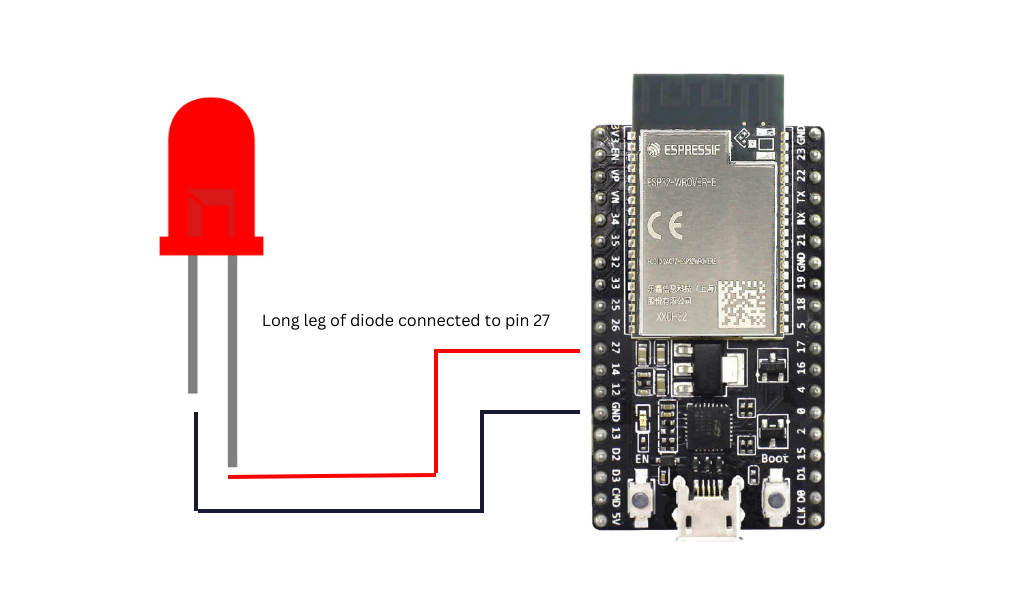
\includegraphics[scale=0.3]{led.png}
  \caption{LED Wiring}
  \label{fig:led}
\end{figure}
\subsection*{Button Input to turn on LED}
Teaches students how to handle input.
\begin{figure}[H]
  \centering
  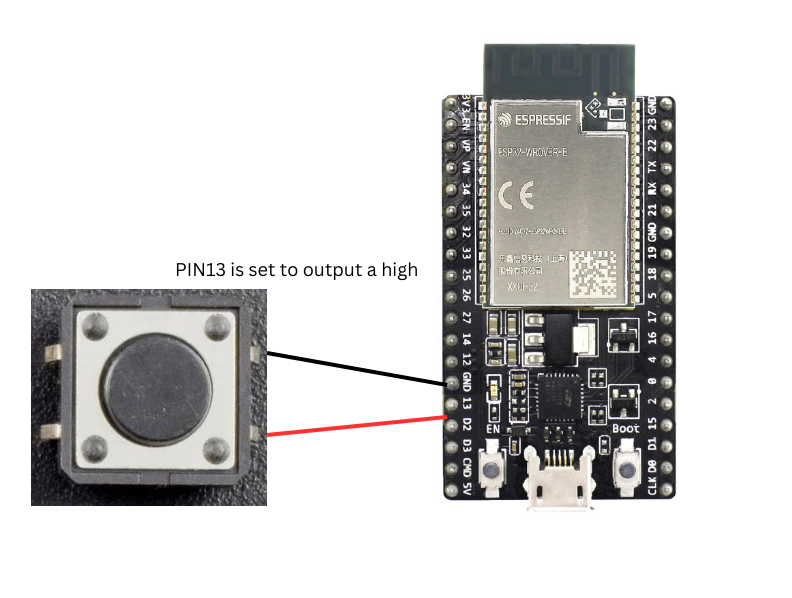
\includegraphics[scale = 0.3]{button.png}
  \caption{Button Wiring}
  \label{fig:button}
\end{figure}
\subsection*{PWM}
PWM for things such as motors and SG90 servos.
\begin{figure}[H]
  \centering
  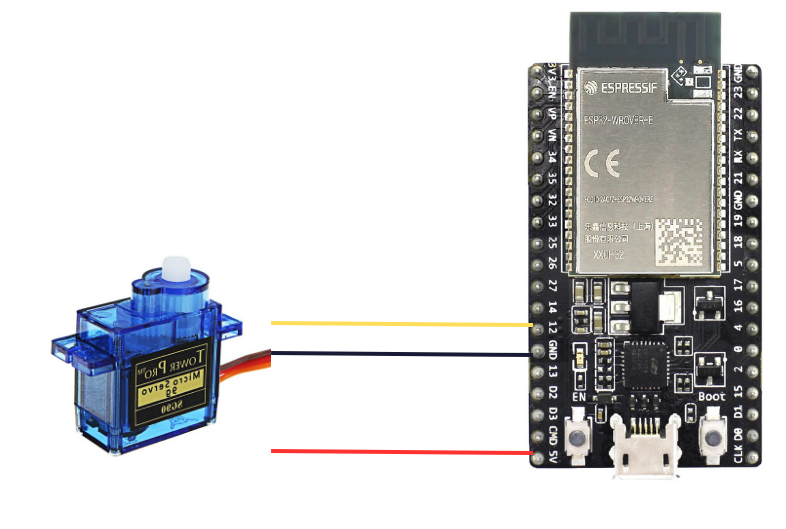
\includegraphics[scale = 0.3]{servo.png}
  \caption{Servo wiring}
  \label{fig:servo}
\end{figure}
\section*{Advanced Lessons}
\subsection*{Wireless Communication}
Wireless communication is essential for remotely operated devices/robotics. 
Although not required, you are usually encouraged to use wireless 
communication in the ENGG1100 and METR2800 group projects.
% Ill need a fact check here cause I didn't do METR2800
% I did not need wireless for METR2800 pretty sure.
Alternatively, many groups use a long USB cable to remotely operate their 
machine - yuck. After this tutorial you will hopefully gain the confidence to blah blah....

\section*{How to program Microcontroller with C}
https://docs.espressif.com/projects/esp-idf/en/latest/esp32/

\end{document}
